%%%%%%%%%%%%%%%%%%%%%%%%%%%%%%%%%%%%%%%%%%%%%%%%%%%%%%%
% Underwriter Cheat Sheet
%
% Created by Stephen J Mildenhall
% (c) 2023
%
%%%%%%%%%%%%%%%%%%%%%%%%%%%%%%%%%%%%%%%%%%%%%%%%%%%%%%%

\documentclass{article}
% general includes
\usepackage[landscape]{geometry}
\usepackage{url}
\usepackage{multicol}
\usepackage{amsmath}
\usepackage{amsfonts}
\usepackage{tikz}
\usepackage{xcolor}
% \usetikzlibrary{decorations.pathmorphing}
\usetikzlibrary{calc}
\usepackage{amsmath}
\usepackage{amssymb}

\usepackage{colortbl}
\usepackage{xcolor}
\usepackage{mathtools}
\usepackage{amsmath,amssymb}
\usepackage{enumitem}

\usepackage[english]{babel}

% fontws
\usepackage{stix}

\advance\topmargin-.8in
\advance\textheight3in
\advance\textwidth3in
\advance\oddsidemargin-1.5in
\advance\evensidemargin-1.5in
\parindent0pt
\parskip2pt
\newcommand{\hr}{\centerline{\rule{3.5in}{1pt}}}

% colors from the logo
% https://color.adobe.com/mythemes?viewTheme
\definecolor{highlightcolora}{HTML}{73171F}
\definecolor{highlightcolorb}{HTML}{CB7C13}
\definecolor{highlightcolorc}{HTML}{168C6B}
\definecolor{highlightcolord}{HTML}{355078}
\definecolor{highlightcolore}{HTML}{263940}

\colorlet{washedcolora}{highlightcolora!20!white}
\colorlet{washedcolorb}{highlightcolorb!20!white}
\colorlet{washedcolorc}{highlightcolorc!20!white}
\colorlet{washedcolord}{highlightcolord!20!white}
\colorlet{washedcolore}{highlightcolore!20!white}

\colorlet{texta}{white}
\colorlet{textb}{white}
\colorlet{textc}{white}
\colorlet{textd}{white}
\colorlet{texte}{white}

% circles for method and static method
\definecolor{hred}{rgb}{1, 0.5, 0.5}
\definecolor{hblue}{rgb}{0.5, 0.5, 1}
\newcommand{\m}{% method
\tikz[baseline=(char.base)]{
    \node[circle, fill=hred, text=white, inner sep=1pt, minimum size=1em] (char) {m};
}\;}
\newcommand{\s}{% static method
\tikz[baseline=(char.base)]{
    \node[circle, fill=hblue, text=white, inner sep=1pt, minimum size=1em] (char) {s};
}\;}


%% TikZ MACROS

% title box - adjust text color as appropriate here
\tikzstyle{fancytitle} =[
    fill=highlightcolor,
    text=textcolor,
    font=\bfseries,
    right=10pt
    ]

% content box
\tikzstyle{mybox} = [
    draw=highlightcolor,
    fill=washedcolor,
    very thick,
    rectangle,
    inner sep=10pt,
    inner ysep=10pt
    ]


\newcommand{\makefooter}{%
% \vfil
% \hfill
\begin{tikzpicture}[remember picture, overlay]
    \node[anchor=south east, inner sep=0pt, outer sep=0pt] at ($(current page.south east) + (-0.125in,0.125in)$) {

        \begin{tikzpicture}
        \node [font=\small, text height=0.75in, align=right, minimum height=0.75in, inner xsep=5pt, inner ysep=0pt] (box){%
            \copyright\ Stephen J Mildenhall \\
            \texttt{aggregate 0.18.0} \\
            2023-07-16
        };
        \node[inner sep=0pt, anchor=north west] at (box.north east) {
            \includegraphics[width=0.75in,height=0.75in,keepaspectratio]{../docs/_static/agg_logo.png}
        };
        \end{tikzpicture}

    };
\end{tikzpicture}
}

\title{Underwriter Cheat Sheet}

% color scheme defeined here - just change the suffixes
\colorlet{highlightcolor}{highlightcolora}
\colorlet{washedcolor}{washedcolora}
\colorlet{textcolor}{texta}

\begin{document}

{\huge{\bf \textbf{\texttt{Underwriter} Class Cheat Sheet}}}

\raggedright The \texttt{Underwriter} call signature follows the corresponding DecL clauses, using prefixes for exposure (including limit sub-clause), severity, occurrence reinsurance, frequency, aggregate reinsurance, and note. \texttt{sev\_xs, sev\_ps} equal \texttt{dsev} outcomes and probabilities, and \texttt{(occ|agg)\_reins} clauses are lists of (share, limit, attachment) triples. \\
 \texttt{\m Severity(name, exp\_el=0, exp\_premium=0, exp\_lr=0, exp\_en=0, exp\_attachment=0, exp\_limit=np.inf}, \\
 \texttt{\phantom{\m}sev\_name='', sev\_a=np.nan, sev\_b=0, sev\_mean=0, sev\_cv=0, sev\_loc=0, sev\_scale=0, sev\_xs=None, sev\_ps=None, sev\_wt=1, sev\_conditional=True, }\\
% \texttt{sev\_pick\_attachments=None, sev\_pick\_losses=None, }\\
 \texttt{\phantom{\m}occ\_reins=None, occ\_kind='', freq\_name='', freq\_a=0, freq\_b=0, freq\_zm=False, freq\_p0=np.nan, agg\_reins=None, agg\_kind='', note='')}${}^{[0]}$

The following tables show all \texttt{\m methods}, and fields or properties (used interchangeably). Comments elucidate the meaning of more obscure entries.


\begin{multicols*}{3}


%------------1. SPECIFICATION & CREATION ---------------
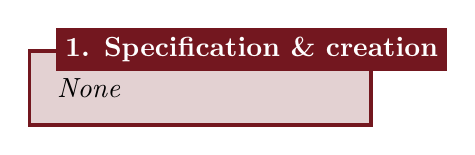
\begin{tikzpicture}
\node [mybox] (box){%
    \begin{minipage}{0.3\textwidth}\raggedright

{\it None }


    \end{minipage}
};
\node[fancytitle] at (box.north west) {1. Specification \& creation};
\end{tikzpicture}


%------------2. UPDATE ---------------
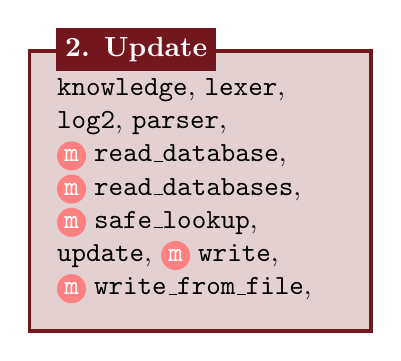
\begin{tikzpicture}
\node [mybox] (box){%
    \begin{minipage}{0.3\textwidth}\raggedright
    
\texttt{knowledge},
\texttt{lexer},
\texttt{log2},
\texttt{parser},
\texttt{\m read\_database},
\texttt{\m read\_databases},
\texttt{\m safe\_lookup},
\texttt{update},
\texttt{\m write},
\texttt{\m write\_from\_file},


    \end{minipage}
};
\node[fancytitle] at (box.north west) {2. Update};
\end{tikzpicture}


%------------ 3. MOMENTS ---------------
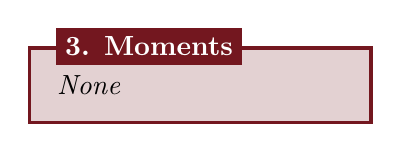
\begin{tikzpicture}
\node [mybox] (box){%
    \begin{minipage}{0.3\textwidth}\raggedright

{\it None }


    \end{minipage}
};
\node[fancytitle] at (box.north west) {3. Moments};
\end{tikzpicture}


%------------ 4. STATISTICAL FUNCTIONS ---------------
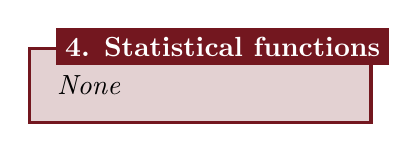
\begin{tikzpicture}
\node [mybox] (box){%
    \begin{minipage}{0.3\textwidth}\raggedright

{\it None }


    \end{minipage}
};
\node[fancytitle] at (box.north west) {4. Statistical functions};
\end{tikzpicture}


\columnbreak


%------------ 5. VALIDATION ---------------
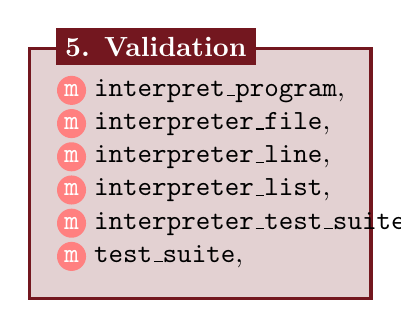
\begin{tikzpicture}
\node [mybox] (box){%
    \begin{minipage}{0.3\textwidth}\raggedright

\texttt{\m interpret\_program},
\texttt{\m interpreter\_file},
\texttt{\m interpreter\_line},
\texttt{\m interpreter\_list},
\texttt{\m interpreter\_test\_suite},
\texttt{\m test\_suite},


    \end{minipage}
};
\node[fancytitle] at (box.north west) {5. Validation};
\end{tikzpicture}


%------------ 6. OUTPUT ---------------
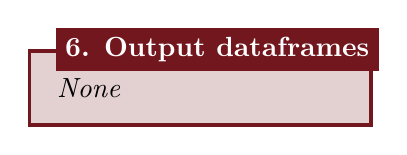
\begin{tikzpicture}
\node [mybox] (box){%
    \begin{minipage}{0.3\textwidth}\raggedright

{\it None }

    \end{minipage}
};
\node[fancytitle] at (box.north west) {6. Output dataframes};
\end{tikzpicture}


%------------ 7. REINSURANCE ---------------
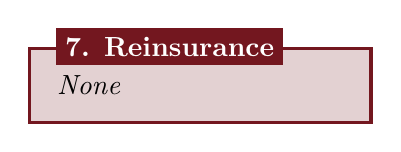
\begin{tikzpicture}
\node [mybox] (box){%
    \begin{minipage}{0.3\textwidth}\raggedright

{\it None }

    \end{minipage}
};
\node[fancytitle] at (box.north west) {7. Reinsurance};
\end{tikzpicture}



\columnbreak


%------------ 8. VISUALIZTION ---------------

\begin{tikzpicture}
\node [mybox] (box){%
    \begin{minipage}{0.3\textwidth}\raggedright

{\it None }


    \end{minipage}
};
\node[fancytitle] at (box.north west) {8. Visualization};
\end{tikzpicture}


%------------ 9. RISK ---------------
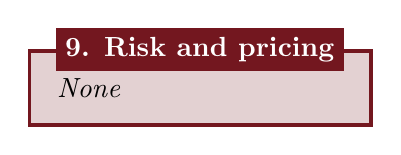
\begin{tikzpicture}
\node [mybox] (box){%
    \begin{minipage}{0.3\textwidth}\raggedright
    
{\it None }

    \end{minipage}
};
\node[fancytitle] at (box.north west) {9. Risk and pricing};
\end{tikzpicture}


%------------  10. APPROXIMATIONS ---------------

\begin{tikzpicture}
\node [mybox] (box){%
    \begin{minipage}{0.3\textwidth}\raggedright

{\it None }

    \end{minipage}
};
\node[fancytitle] at (box.north west) {10. Approximations};
\end{tikzpicture}


%------------ 11. META ---------------
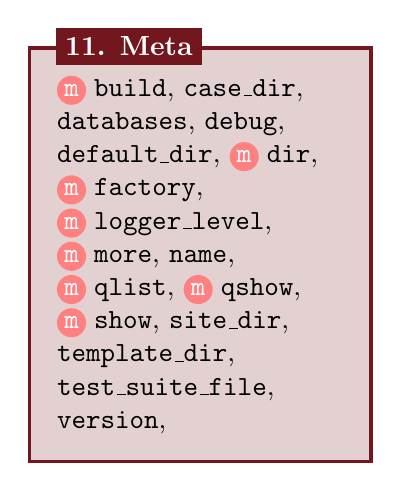
\begin{tikzpicture}
\node [mybox] (box){%
    \begin{minipage}{0.3\textwidth}\raggedright
    
\texttt{\m build},
\texttt{case\_dir},
\texttt{databases},
\texttt{debug},
\texttt{default\_dir},
\texttt{\m dir},
\texttt{\m factory},
\texttt{\m logger\_level},
\texttt{\m more},
\texttt{name},
\texttt{\m qlist},
\texttt{\m qshow},
\texttt{\m show},
\texttt{site\_dir},
\texttt{template\_dir},
\texttt{test\_suite\_file},
\texttt{version},


    \end{minipage}
};
\node[fancytitle] at (box.north west) {11. Meta};
\end{tikzpicture}

\bigskip \raggedright
{\bf Notes:} 

[0]: Arguments \texttt{sev\_pick\_attachments=None, sev\_pick\_losses=None, } omitted; see help. 

[1]: matches \texttt{Portfolio} 

Any vectorizable input accepts numeric or iterable datatypes.  

Abbreviations: gcn=gross (subject), ceded, and net; stats: m=mean, cv=coefficient of variation, sd=standard deviation, var=variance, skew(ness); VaR=value-at-risk


% \vskip .25truein
% FOOTER
\makefooter



\end{multicols*}

\end{document}
